%----------------------------------------------------------------------------------------
%	PACKAGES AND DOCUMENT CONFIGURATIONS
%----------------------------------------------------------------------------------------
\documentclass[11pt]{article}
\usepackage{amsmath} % Required for some math elements
\usepackage[usenames,dvipsnames]{xcolor}
\usepackage{lipsum} 
\usepackage{cite}
\usepackage{graphicx} % Required for the inclusion of images
\usepackage{algorithmic}
\usepackage{array}
\usepackage{bookmark}
\usepackage{listings}
\usepackage{amssymb}
\usepackage{enumitem}
\usepackage[margin=24mm]{geometry}
\usepackage[caption=false, font=footnotesize]{subfig}
\usepackage{multirow}
\usepackage[active,tightpage]{preview}
\usepackage{hyperref} 

\renewcommand{\PreviewBorder}{1in}
\newcommand{\Newpage}{\end{preview}\begin{preview}}

\newlist{steps}{enumerate}{1}
\setlist[steps, 1]{label = Step \arabic*:}

\hypersetup{ %color attributes of citation, link, etc.
    colorlinks=true,
    linkcolor=blue,
    filecolor=gray,      
    urlcolor=blue,
    citecolor=blue,
}

 
\lstdefinelanguage{VHDL}{
    morekeywords=[1]{
        library,use,all,entity,is,port,in,out,end,architecture,of,begin,and,or,Not,downto,ALL
    },
    morekeywords=[2]{
        STD_LOGIC_VECTOR,STD_LOGIC,IEEE,STD_LOGIC_1164,NUMERIC_STD,STD_LOGIC_ARITH,STD_LOGIC_UNSIGNED,std_logic_vector,std_logic
    },
    morecomment=[l]--
}

\definecolor{keyword}{rgb}{0,0.3,0.7}
\definecolor{STD}{rgb}{0.9,0.0,0.7}
\definecolor{comment}{rgb}{0.0,0.6,0.1}

\lstdefinestyle{vhdl}{
   language     = VHDL,
   basicstyle   = \footnotesize\ttfamily,
   keywordstyle = [1]\color{keyword}\bfseries,
   keywordstyle = [2]\color{STD}\bfseries,
   commentstyle = \color{comment}
   breaklines=true,                % sets automatic line breaking
   tabsize=3		                   % sets default tabsize to 2 spaces
}


\newcommand{\matlab}{\textsc{Matlab }} %very important and totally necessary addition

\newcommand\Item[1][]{%
    \ifx\relax#1\relax  \item \else \item[#1] \fi
    \abovedisplayskip=0pt\abovedisplayshortskip=0pt~\vspace*{-\baselineskip}}
%----------------------------------------------------------------------------------------
%	DOCUMENT INFORMATION
%----------------------------------------------------------------------------------------
 
\title{ECEN302 : Integrated Digital Electronics \\ Assignment 1 Submission}
\author{Daniel Eisen : 300447549}
\date{\today}

\begin{document}
\begin{preview}
\maketitle
%----------------------------------------------------------------------------------------
%	DOCUMENT CONTENT
%----------------------------------------------------------------------------------------
\begin{enumerate}
    \item \textbf{Look up the data sheet for the device we are using in the laboratory and then answer the following questions:}

    The device on the Nexys4 DDR and A7 boards if is the Artix-7 100T.
  
    \begin{enumerate}
        \item \textit{How many CLBs are there?}

        There are 7925 CLB's  (15850 logic slice pairs).
    
        \item \textit{How many I/O pins?}

        The max supported single ended I/O is 300, but on the CSG324 package there are \textbf{210} user  available I/O pins. 

        \item \textit{What I/O voltages can be accommodated and how is this configured?}

        1.2V, 1.5V, 1.8V, 2.5V and, 3.3V. These are selected by setting the IOSTANDARD in I/O planning or in the constraints file of your project.
        
        \item \textit{What is the physical footprint?}

        The CSG324 package is 15x15 mm.~

        \item \textit{What does “speed grade” mean?}

        Xilinx defines the 'Speed Grade" of specifically FPGA devices to be a general indication of the timing performance of that device. These are specified as relative rating with a device family. I.e. -1,-2,-3 etc. from slowest to fastest.
        Each speed grade level represents around a 10-15\% performance difference.

    \end{enumerate}

    \item \textbf{With reference to the CLB:}
    \begin{enumerate}
        \item \textit{How is combinatorial logic typically implemented?}

        In an FPGA's CLBs the logic slices contain lookup tables that represent the truth table of the combinatorial logic. These can be chained/cascaded together to construct more complex designs.
        
        \item \textit{What is the main purpose of the flipflops/latches?}

        FF/Latches are primary used to hold the value of an input signal that may be transient long enough to be held, and passed on for further processing. They also allow for synchronizing with a clock cycle.

        \item \textit{What is the carry chain and what is it used for?}
        The carry chain is vertically connecting line between the logic slices (and the LUTs within) of the CLBs. It is a feature that allows for very fast arithmetic operations (add, subtract) throughout the LUTs.
    
        \item \textit{What is the deference between a SLICEM and a SLICEL?}
        
        SLICEM(memory) is a full slice and can be used for bother logic, memory, and shift registers.
        Where SLICEL(logic), can only be used for logic and implementing combinatorial functions. 

        \item \textit{How are the CLBs connected to other CLBs?}
        
        CLB's are joins in a large 'fabric' of programmable interconnect and via the carry chain. The fabric allows for a large number of unique connections and configuration to be designed and constructed. Each CLB is connected to this interconnect through the Switch Matrix to allow for routing to other CLBs and other FPGA resources. 

    \end{enumerate}

    \item \textbf{With regard to FPGA design:}
    \begin{enumerate}
        \item \textit{Describe the principle of pipelining and why it is often necessary?}
        
        Pipelining is separating sections of combinatorial logic up and connecting them through registers. These are synchronized to a shared clock so that every happen at on a edge. This is done because it avoids possible timing errors and allows for the planning/construction/testing to much larger design as it would be much more difficult to do so and to debug the design if it were asynchronous.

        \item \textit{Explain “setup” and “hold” timing?}

        Data is "read" from an incoming signal by latching it on an active clock edge. The \textbf{setup} time if a defined value of the minimum required amount of time before said actives clock edge that the data must be stable (unchanging) to be correctly captured.\\ The \textbf{hold} time is likewise the minimum time that the data must be held after the edge to be successfully captured.  Failure to meet these requirements may cause the wrong data to be latched and/or risk metastability.

    

        \item \textit{What is metastability and what are the two main causes of it?}

        When an output become 'undefined', basically hovering \emph{between} the high and low state for some period of time it is characterised as metastable.
        One cause can be built up propagation delay eventually resulting in setup and hold timing violations.
        Another is if there are two clock domains present, say 2 FF in series each with different clocks, there is the possibility of the two separate clocks transitions resulting in a changing input as it is latched, resulting in a metastable output.


        \item \textit{How do we typically deal with metastability?}

        To solve the previously discussed issue a "Synchronisation Register Chain" can be used to stabilise the output. Practically this is just a D-FF on the output, synced to the same clock domain of FF that is input. This can allow to some internal metastability but satisfying a stable output. 


        \item \textit{Describe the difference between Mealy and Moore FSMs}
            \begin{itemize}
                \item Mealy FSM have an output that is dependant/changes based on both their current input and present state of the machine. This usually results in less discrete states than a Moore FMS. The input dependence also means that the output can change asynchronously.
                \item Moore FSM changer output only due to present state, i.e. a unique state per unique output, and are updated on the clock edge. This means the topology can be slower over all, but more predicable and synchronising.
            \end{itemize}


    \end{enumerate}

    \item \textbf{VHDL design. Compare and Add Circuit.}
    \lstinputlisting[language=VHDL]{../compare_add/compare_add.srcs/sources_1/new/comp_add.vhd}

    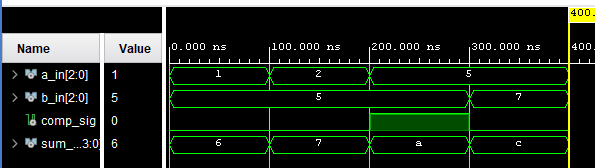
\includegraphics[width=\textwidth]{inc/sim.png}

    \lstinputlisting[language=VHDL]{../compare_add/compare_add.srcs/sim_1/new/comp_add_tb.vhd}
    
    
    \item \textbf{Below is a list of tools or methods that can assist and/or accelerate the development and debugging of code for FPGAs. For each one describe the process and its benefit to the developer.}
    % \item (note: it is expected that you write at least a quarter of an A4 page on each item. Feel free to include pictures).
    \begin{enumerate}
        \item \textit{Schematic generation of synthesized and routed designs}
        When designing for a FPGA project, just writing pure HDL code can make it hard to confirm if the direction and overall logic of the system if to spec or consistent with the logic of the intended feature-set other than a full test/simulation. For this Vivado supplies the Schematic feature to help the developer confirm/visualise their design.

        The first is the schematic generated during RTL Analysis, and this shows a logical view of the code as a representation of the pre-optimized design in terms of generic symbols, such as adders, multipliers, counters, AND gates, and OR gates, that are independent of the targeted device. The exact representation may differ due to the design approach the code is written in, but it served the same purpose to inform the developer as to if the design is correct or to provide an alternate angle to debug any problems.

        The second schematic generated later in the Vivado design flow is provided by running Synthesis and/or implementation. This give the overview/idea/approximation of how the design will be constructed on device, with LUTs and buffers and gives the developer the level of resources that will utilised, i.e. IO, timing, et.

        \item \textit{Test bench simulation}

        During the process of HDL development the code must be tested to verify its function. The Test Bench toolset allows for this testing to be done digitally, without the need to run on device. In fact it enables the developer, through the writing of the HDL test bench code, to produce a repeatable set of stimulus to their FPGA codebase. Allowing for input control, clocking, timing control, in depth error checking and can be transferred between different simulators. 
        
        \begin{center}
            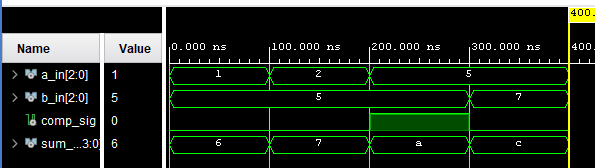
\includegraphics[width=0.69\textwidth]{inc/sim.png}
            \textit{Example of test bench simulation of precise timing and input signal changes}
        \end{center}

        This represents a huge opportunity for rapid increase in development speed not only because simulations do not require full synthesis/implementation but for much larger/complex designed the simulation can provide a much higher level of detail internal information and data about the working of the code and can quickly run through more testing scenarios faster than could be done physically on device.

        \item \textit{Timing analyser}
        
        After HDL is Implelmented, a developer can run the Timing Analyzer. This tool provides a detailed analysis report in the timing performance on the design. Using this tool allows the developer to confirm that the code as implemented:
        \begin{itemize}
            \item Conforms to the constraints and timing requirements of each path.
            \item Show their setup and hold performances, if there are violations and by how much
            \item Can catch any error created by forgetting to constrain certain paths etc 
        \end{itemize}

        Having to ability to gauge at least estimated of the exact performance of a design and to catch any preliminary errors and violations again during the writing of code stage saves time in testing and in later debugging. 

        \item \textit{Integrated Logic Analyzer (ILA)}

        Xilinx provides a customisable IP core in the Vivado Design suite. It can be used be including the design template from the IP catalogue, customising the component by setting number of probes, data width, etc. Then by using the instance template and fleshing out the code to connect it to the modules/ports relevant to what is wanted to be inspected. Using this IP core allows for the developer to get a much deeper and richer understanding of the internal signals of the device under operating conditions than could be possibly obtained physically. It supports terminal interfacing, triggering, pre-setup measurements, comparisons and much more deeper probing features. This rich feature setup and flexibility will be vitally important if working on a larger, complexly interconnected design that may not have a singular inspectable function and debugging requirement the necessitate and more internal view.
\end{enumerate}



\end{enumerate}
\end{preview}
\end{document}  